\begin{orismos}{Ανίσωση}
Ανίσωση ονομάζεται κάθε ανισότητα η οποία περιέχει τουλάχιστον μια μεταβλητή.
\end{orismos}
\begin{itemize}[itemsep=0mm]
\item Ανισώσεις αποτελούν και οι σχέσεις με σύμβολα ανισοϊσότητας $ \leq,\geq $.
\item Κάθε αριθμός που επαληθεύει μια ανίσωση ονομάζεται \textbf{λύση} της. Κάθε ανίσωση έχει λύσεις ένα \textbf{σύνολο αριθμών}.
\item Αν μια ανίσωση έχει λύσεις όλους τους αριθμούς ονομάζεται \textbf{αόριστη}.
\item Αν μια ανίσωση δεν έχει καθόλου λύσεις ονομάζεται \textbf{αδύνατη}.
\item Σχέσεις τις μορφής $ Q(x)\leq P(x)\leq R(x) $ λέγονται \textbf{διπλές ανισώσεις} όπου $ P(x),Q(x),\\R(x) $ αλγεβρικές παρατάσεις. Αποτελείται από δύο ανισώσεις, με κοινό μέλος την παράσταση $ P(x) $, οι οποίες συναληθεύουν.
\item \textbf{Κοινές λύσεις} μιας διπλής ανίσωσης ή δύο ή περισσότερων ανισώσεων ονομάζονται οι αριθμοί που επαληθεύουν όλες τις ανισώσεις συγχρόνως.
\end{itemize}
\Paradeigma{Είδη ανισώσεων}
Σε καθεμία από τις παρακάτω ανισώσεις προκειμένου να προσδιορίσουμε το είδος της, δηλαδή αν είναι αδύνατη ή αόριστη, ελέγχουμε αν υπάρχει αριθμός που να την επαληθεύει.
\begin{itemize}
\item Η ανίσωση $ 0x>2 $ είναι αδύνατη διότι για κάθε τιμή του $ x $ προκύπτει $ 0>2 $ που δεν ισχύει.
\item Η ανίσωση $ 0x\geq2 $ είναι αδύνατη διότι δεν επαληθεύεται καμία από τις σχέσεις $ > $ ή $ = $.
\item Η ανίσωση $ 0x>-2 $ είναι αόριστη διότι για κάθε $ x $ προκύπτει η σχέση $ 0>-2 $ που είναι σωστή.
\item Η ανίσωση $ 0x\geq-2 $ είναι αόριστη διότι ανάμεσα στις σχέσεις $ > $ και $ = $ η σχέση $ > $ είναι αυτή που επαληθεύεται πάντα.
\item Η ανίσωση $ 0x>0 $ είναι αδύνατη διότι προκύπτει πάντα $ 0>0 $ που είναι λάθος.
\item Η ανίσωση $ 0x\geq0 $ είναι αόριστη ή ταυτότητα γιατί από τις $ > $ και $ = $ η ισότητα επαληθεύεται πάντα.
\end{itemize}
Συνεχίζοντας το σκεπτικό αυτό βλέπουμε παρακάτω και τις υπόλοιπες περιπτώσεις αδύνατων και αόριστων ανισώσεων που περιέχουν τις σχέσεις $ < $ και $ \leq $.
\begin{multicols}{2}
\begin{itemize}
\item Η ανίσωση $ 0x<2 $ είναι αόριστη.
\item Η ανίσωση $ 0x\leq2 $ είναι αόριστη.
\item Η ανίσωση $ 0x<-2 $ είναι αδύνατη.
\item Η ανίσωση $ 0x\leq-2 $ είναι αδύνατη.
\item Η ανίσωση $ 0x<0 $ είναι αδύνατη.
\item Η ανίσωση $ 0x\leq 0 $ είναι αόριστη ή ταυτότητα.
\end{itemize}
\end{multicols}


Όμοια με τις εξισώσεις και οι ανισώσεις είναι αλγεβρικές παραστάσεις που περιέχουν πολυώνυμα 1\textsuperscript{ου} βαθμού.\\\\
\thewrhmata


\section{Εξισώσεις - Ανισώσεις 2\tss{ου} βαθμού}
\orismoi
\begin{orismos}{εξίσωση 2\tssLb{ου} βαθμού}
Εξίσωση 2\textsuperscript{ου} βαθμού με έναν άγνωστο ονομάζεται εξίσωση της μορφής :
\[ ax^2+\beta x+\gamma=0\;\;,\;\;a\neq0 \]
\end{orismos} 
\begin{itemize}[itemsep=0mm]
\item Οι πραγματικοί αριθμοί $ a,\beta,\gamma\in\mathbb{R} $ ονομάζονται \textbf{συντελεστές} της εξίσωσης.
\item Ο αριθμός $ \gamma\in\mathbb{R} $ ονομάζεται \textbf{σταθερός όρος}.
\item O πραγματικός αριθμός $ \varDelta=\beta^2-4a\gamma $ ονομάζεται \textbf{διακρίνουσα} του τριωνύμου. Το πρόσημό της μας επιτρέπει να διακρίνουμε το πλήθος των ριζών του τριωνύμου.
\end{itemize}
\begin{orismos}{ανίσωση 2\tssLb{ου} βαθμού}
Ανίσωση 2\textsuperscript{ου} βαθμού με έναν άγνωστο ονομάζεται κάθε ανίσωση της μορφής :
\[ ax^2+\beta x+\gamma>0\;\;.\;\;ax^2+\beta x+\gamma<0 \]
με πραγματικούς συντελεστές $ a,\beta,\gamma\in\mathbb{R} $ και $ a\neq0 $.
\end{orismos}
\thewrhmata
\begin{thewrhma}{λύσεις εξίσωσης 2\textsuperscript{\MakeLowercase{ου}} βαθμού}
Αν $ ax^2+\beta x+\gamma=0 $ με $ a\neq0 $ μια εξίσωση 2\textsuperscript{ου} βαθμού τότε με βάση το πρόσημο της διακρίνουσας έχουμε τις παρακάτω περιπτώσεις για το \textbf{πλήθος} των λύσεων της :
\begin{rlist}
\item Αν $ \varDelta>0 $ τότε η εξίσωση έχει \textbf{δύο άνισες} λύσεις οι οποίες είναι: $ x_{1,2}=\frac{-\beta\pm\!\sqrt{\varDelta}}{2a} $
\item Αν $ \varDelta=0 $ τότε η εξίσωση έχει \textbf{μια διπλή} λύση την $ x=-\frac{\beta}{2a} $.
\item Αν $ \varDelta<0 $ τότε η εξίσωση είναι \textbf{αδύνατη} στο σύνολο $ \mathbb{R} $.
\end{rlist}
\end{thewrhma}
Οι περιπτώσεις αυτές φαίνονται επίσης στον πίνακα :
\begin{center}
\begin{tabular}{ccc}
\hline\textbf{Διακρίνουσα} & \textbf{Πλήθος λύσεων} & \textbf{Λύσεις} \rule[-2ex]{0pt}{5.5ex}\\ 
\hhline{===}\rule[-2ex]{0pt}{7ex} $ \varDelta>0 $ &  2 πραγματικές άνισες λύσεις & $ x_{1,2}=\dfrac{-\beta\pm\!\sqrt{\varDelta}}{2a} $  \\
\rule[-2ex]{0pt}{6.5ex} $ \varDelta=0 $ & 1 διπλή πραγματική λύση & $ x=-\dfrac{\beta}{2a} $\\
\rule[-2ex]{0pt}{6.5ex} $ \varDelta<0 $ & \multicolumn{2}{c}{Καμία πραγματική λύση - Αδύνατη στο $ \mathbb{R} $}\\
\hline 
\end{tabular}\captionof{table}{Λύσεις εξίσωσης 2\tss{ου} βαθμού}
\end{center}
\begin{thewrhma}{Τύποι Vieta}
Έστω $ ax^2+\beta x+\gamma=0 $ με $ a\neq0 $ μια εξίσωση 2\textsuperscript{ου} βαθμού. Αν $ x_1,x_2 $ είναι οι λύσεις της εξίσωση τότε το άθροισμα $ S $ και το γινόμενό τους $ P $ δίνονται από τους τύπους :
\[ S=x_1+x_2=-\dfrac{\beta}{a}\;\;,\;\;P=x_1\cdot x_2=\dfrac{\gamma}{a} \]
οι οποίοι ονομάζονται τύποι του Vieta.
\end{thewrhma}
\begin{thewrhma}{Παραγοντοποίηση τριωνύμου}
Για τη μετατροπή ενός τριωνύμου $ ax^2+\beta x+\gamma\;\;\textrm{με}\;\;a\neq0 $ σε γινόμενο παραγόντων διακρίνουμε τις εξής περιπτώσεις :
\begin{enumerate}[itemsep=0mm]
\item Αν η διακρίνουσα του τριωνύμου είναι θετική $\left( \varDelta>0\right)  $ τότε το τριώνυμο παραγοντοποιείται ως εξής \[ ax^2+\beta x+\gamma=a(x-x_1)(x-x_2) \]
όπου $ x_1,x_2 $ είναι οι ρίζες του τριωνύμου.
\item Αν η διακρίνουσα είναι μηδενική $\left( \varDelta=0\right)  $ τότε το τριώνυμο παραγοντοποιείται ως εξής : \[ ax^2+\beta x+\gamma=a\left(x-x_0\right)^2=a\left(x+\frac{\beta}{2a}\right)^2  \]
όπου $ x_0 $ είναι η διπλή ρίζα του τριωνύμου.
\item Αν η διακρίνουσα είναι αρνητική $\left( \varDelta<0\right)  $ τότε το τριώνυμο δεν γράφεται ως γινόμενο πρώτων παραγόντων. Εναλλακτικά όμως μπορεί να γραφεί : \[ ax^2+\beta x+\gamma=a\left[\left(x+\frac{\beta}{2a}\right)^2+\frac{|\varDelta|}{4a^2}\right]  \]
\end{enumerate}
\end{thewrhma}
\begin{thewrhma}{Πρόσημο τριωνύμου}
Για το πρόσημο των τιμών ενός τριωνύμου $ ax^2+\beta x+\gamma $ ισχύουν οι παρακάτω κανόνες.
\begin{enumerate}[itemsep=0mm]
\item Αν η διακρίνουσα είναι θετική $\left( \varDelta>0\right)  $ τότε το τριώνυμο είναι
\begin{alist}
\item ομόσημο του συντελεστή $ a $ στα διαστήματα που βρίσκονται έξω από τις ρίζες $ x_1,x_2 $.
\item ετερόσημο του $ a $ στο διάστημα ανάμεσα στις ρίζες.
\item ίσο με το μηδέν στις ρίζες.
\end{alist}
\end{enumerate}
\begin{center}
\begin{tikzpicture}
\tikzset{t style/.style = {style = dashed}}
\tkzTabInit[color,lgt=3,espcl=2,colorC = \xrwma!30,
colorL = \xrwma!10,
colorV = \xrwma!30]%
{$x$ / .8,$ax^2+\beta x+\gamma$ /1.2}%
{$-\infty$,$x_1$,$x_2$,$+\infty$}%
\tkzTabLine{ , \genfrac{}{}{0pt}{0}{\text{Ομόσημο}}{ \text{του } a}, z
, \genfrac{}{}{0pt}{0}{\text{Ετερόσημο}}{ \text{του } a}, z
, \genfrac{}{}{0pt}{0}{\text{Ομόσημο}}{ \text{του } a}, }
\end{tikzpicture}\captionof{table}{Πρόσημα τριωνύμου με $ \varDelta>0 $}
\end{center}
\begin{enumerate}[itemsep=0mm,start=2]
\item Αν η διακρίνουσα είναι μηδενική $\left( \varDelta=0\right)  $ τότε το τριώνυμο είναι
\begin{alist}
\item ομόσημο του συντελεστή $ a $ στα διαστήματα που βρίσκονται δεξιά και αριστερά της ρίζας $ x_0 $.
\item ίσο με το μηδέν στη ρίζα.
\end{alist}
\end{enumerate}
\begin{center}
\begin{tikzpicture}
\tikzset{t style/.style = {style = dashed}}
\tkzTabInit[color,lgt=3,espcl=2,colorC = \xrwma!30,
colorL = \xrwma!10,
colorV = \xrwma!30]%
{$x$ / .8,$ax^2+\beta x+\gamma$ /1.2}%
{$-\infty$,$x_0$,$+\infty$}%
\tkzTabLine{ , \genfrac{}{}{0pt}{0}{\text{Ομόσημο}}{ \text{του } a}, z
, \genfrac{}{}{0pt}{0}{\text{Ομόσημο}}{ \text{του } a}, }
\end{tikzpicture}\captionof{table}{Πρόσημα τριωνύμου με $ \varDelta=0 $}
\end{center}
\begin{enumerate}[itemsep=0mm,start=3]
\item Αν η διακρίνουσα είναι αρνητική $\left( \varDelta<0\right)  $ τότε το τριώνυμο είναι
ομόσημο του συντελεστή $ a $ για κάθε $ x\in\mathbb{R}$.
\end{enumerate}
\begin{center}
\begin{tikzpicture}
\tikzset{t style/.style = {style = dashed}}
\tkzTabInit[color,lgt=3,espcl=3.9,colorC = \xrwma!30,
colorL = \xrwma!10,
colorV = \xrwma!30]%
{$x$ / .8,$ax^2+\beta x+\gamma$ /1.2}%
{$-\infty$,$+\infty$}%
\tkzTabLine{, \genfrac{}{}{0pt}{0}{\text{Ομόσημο}}{ \text{του } a}, }
\end{tikzpicture}\captionof{table}{Πρόσημα τριωνύμου με $ \varDelta<0 $}
\end{center}
\end{thewrhma}
\section{Εξισώσεις - Ανισώσεις 3\tss{ου+} βαθμού}
\orismoi
\begin{orismos}{Πολυωνυμική εξίσωση - ανίσωση}
Πολυωνυμική εξίσωση ν-οστού βαθμού ονομάζεται κάθε πολυωνυμική εξίσωση της οποίας η αλγεβρική παράσταση είναι πολυώνυμο ν-οστού βαθμού.
\[ a_\nu x^\nu+a_{\nu-1}x^{\nu-1}+\ldots+a_1x+a_0=0 \]
όπου $ a_\kappa\in\mathbb{R}\;\;,\;\;\kappa=0,1,2,\ldots,\nu $.
\end{orismos}
\textbf{Ρίζα} μιας πολυωνυμικής εξίσωσης ονομάζεται η ρίζα του πολυωνύμου της εξίσωσης. Ομοίως, μια πολυωνυμική ανίσωση θα είναι της μορφής:
\[ a_\nu x^\nu+a_{\nu-1}x^{\nu-1}+\ldots+a_1x+a_0\gtrless0 \]\\
Για να μπορέσουμε να λύσουμε εξισώσεις και ανισώσεις 3\tss{ου+} βαθμού θα προσπαθήσουμε με κατάλληλες παραγοντοποιήσεις να φτιάξουμε γινόμενο πολυωνύμων 1\textsuperscript{ου} βαθμού και 2\textsuperscript{ου} βαθμού. \\Μια χρήσιμη μέθοδος παραγοντοποίησης είναι το σχήμα \textbf{Horner}  \\\\
\section{Κλασματικές - Άρρητες εξισώσεις και ανισώσεις}
\orismoi
\begin{orismos}{Κλασματική εξίσωση}
Κλασματική ονομάζεται μια εξίσωση η οποία περιέχει τουλάχιστον μια ρητή αλγεβρική παράσταση. Γενικά έχει τη μορφή :
\[ \dfrac{P(x)}{Q(x)}+R(x)= 0\]
όπου $ P(x),Q(x),R(x) $ πολυώνυμα με $ Q(x)\neq0 $.
\end{orismos}
\Orismos{Άρρητη εξίσωση}
Άρρητη ονομάζεται κάθε εξίσωση που περιέχει τουλάχιστον μια άρρητη αλγεβρική παράσταση. Θα είναι
\[ \sqrt[\nu]{P(x)}+Q(x)=0 \]
όπου $ P(x),Q(x) $ πολυώνυμα με $ P(x)\geq0 $. Όμοια, μια άρρητη ανίσωση θα είναι:
\[ \sqrt[\nu]{P(x)}+Q(x)\gtrless0 \]
\section{Εξισώσεις - Ανισώσεις διαφόρων ειδών}
\orismoi
\begin{orismos}{διωνυμη εξίσωση}
Διώνυμη εξίσωση ονομάζεται κάθε πολυωνυμική εξίσωση η οποία περιέχει πολυώνυμο με 2 όρους. Θα είναι της μορφής :
\[ x^\nu=a\qquad\textrm{ή}\qquad x^\nu=a^\nu \] όπου  $ \nu\in\mathbb{N}\textrm{ και }a\in\mathbb{R} $.
\end{orismos}
\begin{orismos}{Διτετραγωνη εξισωση}
Διτετράγωνη ονομάζεται κάθε εξίσωση 4\textsuperscript{ου} βαθμού της μορφής :
\[ ax^4+\beta x^2+\gamma=0 \]
με $ a,\beta,\gamma\in\mathbb{R}\;,\;a\neq0 $ η οποία έχει μόνο άρτιες δυνάμεις του $ x $. Οι εκθέτες του τριωνύμου είναι διπλάσιοι απ' αυτούς της εξίσωσης 2\textsuperscript{ου} βαθμού.
\end{orismos}
\thewrhmata
\begin{thewrhma}{εξισωσεισ με απολυτεσ τιμεσ}
Οι βασικές μορφές των εξισώσεων με απόλυτες τιμές είναι οι ακόλουθες :
\begin{enumerate}[itemsep=0mm]
\item Για κάθε εξίσωση της μορφής $ |x|=a $ διακρίνουμε τις παρακάτω περιπτώσεις για τις λύσεις της :
\begin{rlist}[itemsep=0mm]
\item Αν $ a>0 $ τότε η εξίσωση έχει 2 αντίθετες λύσεις : $ |x|=a\Leftrightarrow x=\pm a $
\item Αν $ a=0 $ τότε η εξίσωση έχει λύση το 0 : $ |x|=0\Leftrightarrow x=0 $
\item Αν $ a<0 $ τότε η εξίσωση είναι αδύνατη.
\end{rlist}
\item Για τις εξισώσεις της μορφής $ |x|=|a| $ ισχύει : $ |x|=|a|\Leftrightarrow x=\pm a $
\item Με τη βοήθεια των παραπάνω, μπορούμε να λύσουμε και εξισώσεις της μορφής $ \left|f(x) \right|=g(x)  $ και $ \left|f(x) \right| =\left|g(x) \right|  $ όπου $ f(x),g(x) $ αλγεβρικές παραστάσεις :
\begin{rlist}
\item $ \left|f(x) \right|=g(x)\Leftrightarrow f(x)=\pm g(x) $ όπου θα πρέπει να ισχύει $ g(x)\geq 0 $.
\item $ \left|f(x) \right|=\left| g(x)\right| \Leftrightarrow f(x)=\pm g(x) $.
\end{rlist}
\end{enumerate}
\end{thewrhma}

\begin{thewrhma}{εξισωσεισ τησ μορφησ {\MakeLowercase{$\mathbold {x^\nu=a }$}}}
Για τις λύσεις των εξισώσεων της μορφής $ x^\nu=a $ διακρίνουμε τις παρακάτω περιπτώσεις για το είδος του εκθέτη $ \nu $ και του πραγματικού αριθμού $ a $.
\begin{enumerate}[itemsep=0mm]
\item	Για $ \nu $ άρτιο έχουμε :
\begin{enumerate}[itemsep=0mm,label=\roman*.]
\item Αν $ a\geq0 $ τότε η εξίσωση έχει 2 λύσεις αντίθετες :
$ x^\nu=a\Leftrightarrow x=\pm \sqrt[\nu]{a} $
\item Αν $ a<0 $ τότε η εξίσωση είναι αδύνατη.
\end{enumerate}
\item Για $ \nu $ περιττό έχουμε :
\begin{enumerate}[itemsep=0mm,label=\roman*.]
\item Αν $ a\geq0 $ τότε η εξίσωση έχει 1 θετική λύση : $ x^\nu=a\Leftrightarrow x=\sqrt[\nu]{a} $
\item Αν $ a<0 $ τότε η εξίσωση έχει 1 αρνητική λύση : $ x^\nu=a\Leftrightarrow x=-\!\sqrt[\nu]{|a|} $
\end{enumerate}
\end{enumerate}
\end{thewrhma}
Οι λύσεις των εξισώσεων της μορφής $ x^\nu=a $ φαίνονται στο παρακάτω διάγραμμα για κάθε μια από τις περιπτώσεις που αναφέραμε :
\begin{center}
\begin{tikzpicture}[box/.style={minimum height=.5cm,draw,rounded corners,minimum width=1.2cm,align=center},y=1cm]
\node[box] (eks) at (0,4) {{\footnotesize Αρχική εξίσωση}\\{\footnotesize $ x^\nu=a $}};
\node[box] (a) at (-2,3) {{\footnotesize $ \nu $ άρτιος}};
\node[box] (p) at (2,3) {{\footnotesize $ \nu $ περιττός}};
\node[box] (th1) at (-3,2) {{\footnotesize $ a\geq0 $}};
\node[box] (ar1) at (-1,2) {{\footnotesize $ a<0$}};
\node[box] (th2) at (1,2) {{\footnotesize $ a\geq0 $}};
\node[box] (ar2) at (3,2) {{\footnotesize $ a<0 $}};
\node[box] (ly1) at (-3,1) {{\footnotesize $ x=\pm \sqrt[\nu]{a} $}};
\node[box] (ly2) at (-1,1) {{\footnotesize αδύνατη}};
\node[box] (ly3) at (1,1) {{\footnotesize $ x=\sqrt[\nu]{a} $}};
\node[box] (ly4) at (3,1) {{\footnotesize $ x=-\!\sqrt[\nu]{|a|} $}};
\draw[-] (eks.270) -- (0,3.5);
\draw[-latex] (eks.270) -- (0,3.5) -- (-2,3.5) -- (a.90);
\draw[-latex] (0,3.5) -- (2,3.5) -- (p.90);
\draw[-latex] (a.270) -- (-2,2.5) -- (-3,2.5) -- (th1.90);
\draw[-latex] (-2,2.5) -- (-1,2.5) -- (ar1.90);
\draw[-latex] (p.270) -- (2,2.5) -- (1,2.5) -- (th2.90);
\draw[-latex] (2,2.5) -- (3,2.5) -- (ar2.90);
\draw[-latex] (th1.270)  -- (ly1.90);
\draw[-latex] (ar1.270)  -- (ly2.90);
\draw[-latex] (th2.270)  -- (ly3.90);
\draw[-latex] (ar2.270)  -- (ly4.90);
\node at (-6,4) {Αρχική εξίσωση};\draw[-latex] (-4.6,4)--(-4,4) ;
\node at (-6,3) {Εκθέτης};\draw[-latex] (-4.6,3)--(-4,3) ;
\node at (-6,2) {Αποτέλεσμα};\draw[-latex] (-4.6,2)--(-4,2) ;
\node (Eksiswsh) at (-6,1) {Λύσεις};\draw[-latex] (-4.6,1)--(-4,1) ;
\end{tikzpicture}
\end{center}
\Thewrhma{εξισωσεισ τησ μορφησ {\MakeLowercase{$ \mathbold{x^\nu=a^\nu} $}}}
Για τις λύσεις των εξισώσεων της μορφής $ x^\nu=a^\nu $ όπου $ \nu\in\mathbb{N^*} $ θα ισχύουν τα παρακάτω :
\begin{rlist}
\item Αν $ \nu $ άρτιος τότε η εξίσωση έχει δύο αντίθετες λύσεις : $ x^\nu=a^\nu\Leftrightarrow x=\pm a $
\item Αν $ \nu $ περιττός τότε η εξίσωση έχει μια λύση : $ x^\nu=a^\nu\Leftrightarrow x=a $
\end{rlist}
Οι λύσεις των εξισώσεων αυτών φαίνονται στο αντίστοιχο διάγραμμα :
\begin{center}
\begin{tikzpicture}[box/.style={minimum height=.5cm,draw,rounded corners,minimum width=1.2cm,align=center},y=1cm]
\node[box] (eks) at (0,4) {{\footnotesize Αρχική εξίσωση}\\{\footnotesize $ x^\nu=a^\nu $}};
\node[box] (a) at (-2,3) {{\footnotesize $ \nu $ άρτιος}};
\node[box] (p) at (2,3) {{\footnotesize $ \nu $ περιττός}};
\node[box] (ap1) at (-2,2) {{\footnotesize $ x=\pm a $}};
\node[box] (ap2) at (2,2) {{\footnotesize $ x=a $}};
\draw (eks.270) -- (0,3.5);
\draw[-latex] (eks.270) -- (0,3.5) -- (-2,3.5) -- (a.90);
\draw[-latex] (0,3.5) -- (2,3.5) -- (p.90);
\draw[-latex] (a.270) -- (ap1.90);
\draw[-latex] (p.270) -- (ap2.90);
\node at (-5,4) {Αρχική εξίσωση};\draw[-latex] (-3.6,4)--(-3,4) ;
\node at (-5,3) {Εκθέτης};\draw[-latex] (-3.6,3)--(-3,3) ;
\node (Eksiswsh) at (-5,2) {Λύσεις};\draw[-latex] (-3.6,2)--(-3,2) ;
\end{tikzpicture}
\end{center}
\newpage
\Lymena

\begin{Methodos}[Ανισώσεις 1\tssLb{ου} βαθμού]{9cm}
\textbf{Βήματα}
\begin{enumerate}[itemsep=0mm]
\item Τα βήματα που ακολουθούμε είναι τα ίδια με την επίλυση εξισώσεων 1ου βαθμού με τη μόνη διαφορά να είναι στην διαίρεση με τον συντελεστή του αγνώστου.
\item Στο τελευταίο βήμα,όταν διαιρέσουμε με το συντελεστή του αγνώστου πρέπει να γνωρίζουμε το πρόσημό του:
\begin{itemize}
\item αν είναι θετικό τότε η φορά της ανίσωσης παραμένει η ίδια.
\item αν είναι αρνητικό πρέπει να αλλάξουμε την φορά της ανίσωσης.
\end{itemize}
\end{enumerate}
\end{Methodos}
\lysh\\
\begin{parat}{5cm}
Δεν έχει σημασία σε ποιο μέλος θα βρίσκονται οι γνωστοί και σε ποιο οι άγνωστοι. Συνήθως στο αριστερό βάζουμε τους γνωστούς και στο δεξί τους γνωστούς.
\end{parat}
\begin{prosoxi}{5cm}
Προσέχω πολύ κάθε φορά που αλλάζω μέλος κάποιον όρο πρέπει να του αλλάξω και πρόσημο.
\end{prosoxi}
\begin{Methodos}[Εξισώσεις 2\tssLb{ου} βαθμού]{9cm}
Κάθε εξίσωση 2\tss{ου} βαθμού της μορφής 
\[ ax^2+\beta x+\gamma=0\ \ ,\ \ a\neq 0 \]
λύνεται ακολουθώντας τα παρακάτω βήματα.
\begin{bhma}
\item\textbf{Εύρεση διακρίνουσας}\\
Υπολογίζουμε τη διακρίνουσα του τριωνύμου δηλαδή τον πραγματικό αριθμό $ \varDelta=\beta^2-4a\gamma $.
\item\textbf{Λύσεις}\\
Διακρίνουμε τις ακόλουθες περιπτώσεις
\begin{itemize}
\item Αν $ \varDelta>0 $ τότε η εξίσωση έχει δύο λύσεις που δίνονται από τον τύπο $ x_{1,2}=\frac{-\beta\pm\sqrt{\varDelta}}{2a} $
\item Αν $ \varDelta=0 $ η εξίσωση έχει μια διπλή λύση η οποία θα είναι
$ x=-\frac{\beta}{2a} $
\item Αν $ \varDelta<0 $ τότε η εξίσωση είναι αδύνατη.
\end{itemize}
\end{bhma}
\end{Methodos}
\Paradeigma{Εξίσωση 2\tss{ου} βαθμού}
\bmath{Να λυθούν οι παρακάτω εξισώσεις.
\begin{multicols}{3}
\begin{alist}
\item $ x^2-5x+4=0 $
\item $ x^2-6x+9=0 $
\item $ x^2+2x+3=0 $
\end{alist}
\end{multicols}}
\lysh
\begin{alist}
\item Οι συντελεστές της εξίσωσης είναι $ a=1,\beta=-5 $ και $ \gamma=4 $.Η διακρίνουσα λοιπόν θα ισούται με
\[ \varDelta=\beta^2-4a\gamma=(-5)^2-4\cdot 1\cdot 4=25-16=9>0 \]
οπότε η εξίσωση θα έχει δύο λύσεις. Αυτές σύμφωνα με τον παραπάνω τύπο θα είναι
\[ x_{1,2}=\frac{-\beta\pm\sqrt{\varDelta}}{2a}=\frac{-(-5)\pm\sqrt{9}}{2\cdot 1}=\frac{5\pm 3}{2} \]
επομένως θα έχουμε
\[ x_1=\frac{5+3}{2}=\frac{8}{2}=4\ \ \textrm{και}\ \ x_2=\frac{5-3}{2}=\frac{2}{2}=1 \]
\item Ομοίως με το προηγούμενο παράδειγμα, με συντελεστές $ a=1,\beta=-6 $ και $ \gamma=9 $ η διακρίνουσα του τριωνύμου θα είναι
\[ \varDelta=\beta^2-4a\gamma=(-6)^2-4\cdot1\cdot9=36-36=0 \]
συνεπώς η εξίσωση έχει μια διπλή λύση η οποία θα ισούται με \[ x=-\frac{\beta}{2a}=-\frac{-6}{2\cdot 1}=3 \]
\item Οι συντελεστές του πολυωνύμου είναι $ a=1,\beta=2 $ και $ \gamma=3 $. Έχουμε λοιπόν ότι
\[ \varDelta=\beta^2-4a\gamma=2^2-4\cdot1\cdot3=4-12=-8<0 \] επομένως η εξίσωση είναι αδύνατη.
\end{alist}
\begin{Methodos}[Ανισώσεις 2\tss{ου} βαθμού]{9cm}
Για να λυθεί μια ανίσωση 2\tss{ου} βαθμού ακολουθούμε τα επόμενα βήματα.
\begin{bhma}
\item\textbf{Διακρίνουσα}\\
Υπολογίζουμε τη διακρίνουσα του τριωνύμου.
\item \textbf{Ρίζες}\\
Αν $ \varDelta\geq 0 $ τότε υπολογίζουμε τις ρίζες του τριωνύμου.
\item \textbf{Πίνακας προσήμων}\\
Σχεδιάζουμε τον πίνακα προσήμων όπως τον είδαμε στο θεώρημα ... ανάλογα με το πρόσημο της διακρίνουσας. Στη συνέχεια συμπληρώνουμε τα πρόσημα σύμφωνα με τον αντίστοιχο κανόνα.
\item\textbf{Λύσεις ανίσωσης}\\
Επιλέγουμε από τον πίνακα, τα διαστήματα των τιμών του $ x $ για τα οποία επαληθεύεται η ανίσωση.
\end{bhma}
\end{Methodos}
\Paradeigma{Ανίσωση 2\tss{ου} βαθμού}
\bmath{Να λυθούν οι παρακάτω ανισώσεις
\begin{multicols}{3}
\begin{alist}
\item $ x^2-4x+3>0 $
\item $ x^2-6x+9>0 $
\item $ x^2+2x+3>0 $
\item $ x^2-7x+12\leq0 $
\item $ -x^2+8x-16>0 $
\item $ x^2+x+2<0 $
\end{alist}
\end{multicols}}
\lysh
\begin{alist}
\item Για τον υπολογισμό της διακρίνουσας έχουμε $ a=1,\beta=-4 $ και $ \gamma=3 $. Είναι λοιπόν
\[ \varDelta=\beta^2-4a\gamma=(-4)^2-4\cdot1\cdot3=16-12=4>0 \]
άρα το τριώνυμο έχει δύο ρίζες. Αυτές είναι
\[ x_{1,2}=\frac{-\beta\pm\sqrt{\varDelta}}{2a}=\frac{-(-4)\pm\sqrt{4}}{2\cdot 1}=\frac{4\pm 2}{2} \]
δηλαδή \[ x_1=\frac{4+2}{2}=3\ \ \textrm{και}\ \ x_2=\frac{4-2}{2}=1 \]
Στη συνέχεια σχηματίζουμε τον πίνακα προσήμων τοποθετώντας στον άξονα τις ρίζες $ 1,3 $. Με τη βοήθεια του πίνακα αναζητούμε τις τιμές του $ x $ ώστε, σύμφωνα με την ανίσωση, το τριώνυμο να είναι θετικό
\begin{center}
\begin{tikzpicture}
\tikzset{t style/.style = {style = dashed}}
\tkzTabInit[color,lgt=3,espcl=2,colorC = \xrwma!30,
colorL = \xrwma!10,
colorV = \xrwma!30]%
{$x$ / .8,$ x^2-4x+3 $/ 0.8}
{$-\infty$,$1$,$3$,$+\infty$}
\tkzTabLine{ ,+, z, -, z, +, }
\end{tikzpicture}
\end{center}
οπότε οι λύσεις της ανίσωσης είναι $ x\in(-\infty,1)\cup(3,+\infty) $.
\end{alist}
\begin{Methodos}[Εξισώσεις 3\tssLb{ου}+ βαθμού]{9cm}
Για την επίλυση εξίσωσης 3\tss{ου} βαθμού ή μεγαλύτερου, στην οποία οι συντελεστές του πολυωνύμου είναι ακέραιοι ακολουθούμε τα παρακάτω βήματα.
\begin{bhma}
\item\textbf{Πιθανές ακέραιες ρίζες - Εύρεση ρίζας}\\
Από τις πιθανές ακέραιες ρίζες του $ P(x) $ που είναι οι διαιρέτες του σταθερού όρου, βρίσκουμε ποιος αριθμός είναι όντως ρίζα του.
\item \textbf{Σχήμα Horner - Παραγοντοποίηση}\\
Σχηματίζουμε και συμπληρώνουμε το σχήμα Horner με τη ρίζα που βρήκαμε. Παραγοντοποιούμε το πολυώνυμο ως εξής:
\[ P(x)=(x-\rho)\pi(x) \]
όπου $ \pi(x) $ είναι το πηλίκο.
\item \textbf{Λύση εξίσωσης}\\
Αν το πολυώνυμο $ \pi(x) $ είναι δευτέρου βαθμού τότε λύνουμε στη θέση της εξίσωσης $ P(x)=0 $ την ισοδύναμη εξίσωση
\[ (x-\rho)\pi(x)=0 \]
Αν είναι 3\tss{ου} βαθμού ή μεγαλύτερου τότε το παραγοντοποιούμε ακολουθώντας τα δύο προηγούμενα βήματα έως ότου οι παράγοντες να είναι πρωτοβάθμιοι ή δευτεροβάθμιοι.	
\end{bhma}
\end{Methodos}
\Paradeigma{Εξίσωση 3\tssLb{ου} βαθμού}
\bmath{Να λυθεί η παρακάτω εξίσωση
\[ x^3-3x^2-6x+8=0 \]}
\lysh\\
Ξεκινάμε ονομάζοντας $ P(x) $ το πολυώνυμο 3\tss{ου} βαθμού στο πρώτο μέλος της εξίσωσης. Οι πιθανές ακέραιες ρίζες του είναι οι $ \pm1, \pm2, \pm 3 $ και $ \pm 6 $. Απ' αυτές μια ρίζα είναι ο αριθμός $ 1 $ καθώς
\[ P(1)=1^3-3\cdot1^2-6\cdot 1+8=1-3-6+8=0 \]
Συνεπώς θα γίνει σχήμα Horner με ρίζα τον αριθμό $ \rho=1 $
\begin{center}
\horner{1,-3,-6,8}{1}
\end{center}
\wrapr{-5mm}{7}{5cm}{-5mm}{\begin{parat}{5cm}
Το πλήθος των στηλών στο σχήμα Horner για ένα πολυώνυμο $ n- $οστού βαθμού είναι $ n+1 $.
\end{parat}}{
που θα μας δώσει ως πηλίκο το πολυώνυμο $ \pi(x)=x^2-2x+8 $. Το πολυώνυμο $ P(x) $ παραγοντοποιείται ως εξής $ P(x)=(x-1)(x^2-2x+8) $ και έτσι η αρχική εξίσωση θα γραφτεί
\begin{gather*}
P(x)=0\Leftrightarrow (x-1)(x^2-2x+8)=0\Leftrightarrow\\
x-1=0\ \ \textrm{ή}\ \ x^2-2x+8=0
\end{gather*}
Λύνουμε λοιπόν την πρωτοβάθμια και δευτεροβάθμια εξίσωση στις οποίες καταλήξαμε και προκύπτουν έτσι οι λύσεις της αρχικής εξίσωσης $ x=1, x=-2 $ και $ x=4 $.}\\\\\\
\Paradeigma{Εξίσωση 4\tssLb{ου} βαθμού}
\bmath{Να λυθεί η εξίσωση
\[ x^4-9x^2-4x+12=0 \]}
\lysh\\
Όπως και προηγουμένως ονομάζουμε $ P(x) $ το πολυώνυμο του οποίου πιθανές ακέραιες ρίζες είναι οι $ \pm1, \pm 2,\pm 3$  $\pm4, \pm6 $ και $ \pm12 $. Μια ρίζα από τους αριθμούς αυτούς είναι η $ x=-2 $ διότι
\[ P(-2)=(-2)^4-9(-2)^2-4(-2)+12=16-36+8+12=0 \]
Συμπληρώνουμε λοιπόν το σχήμα Horner για το πολυώνυμο $ P(x) $ με ρίζα τον αριθμό $ \rho=-2 $  και έχουμε
\begin{center}
\horner{1,0,-9,-4,12}{-2}
\end{center}
\wrapr{-5mm}{7}{5cm}{-5mm}{\begin{prosoxi}{5cm}
Αν από το πολυώνυμο $ P(x) $ λείπουν όροι, τότε οι συντελεστές τους συμπληρώνονται με $ 0 $ στο σχήμα Horner.
\end{prosoxi}}{Το πηλίκο της διαίρεσης είναι το $ \pi_1(x)=x^3-2x^2-5x+6 $ και η παραγοντοποίηση έχει ως εξής:
\begin{equation}\label{parad:eksiswsh_4ou}
P(x)=(x+2)\cdot\pi_1(x)=(x+2)\left( x^3-2x^2-5x+6\right)
\end{equation}
Καθώς το $ \pi_1 $ είναι 3\tss{ου} βαθμού τότε θα χρειαστεί να παραγοντοποιηθεί και αυτό με τη χρήση του σχήματος Horner. Εύκολα βλέπουμε ότι μια ρίζα του είναι η $ x=1 $ και έτσι θα έχουμε\\\\
\phantom{.}\hspace{3cm}\horner{1,-2,-5,6}{1}}\\\\\\
Το νέο πηλίκο που προκύπτει είναι δευτέρου βαθμού και ισούται με $ \pi_2(x)=x^2-x-6 $ άρα το $ \pi_1(x) $ παραγοντοποιείται ως εξής: $ \pi_1(x)=(x-1)\left( x^2-x-6\right)  $. Σύμφωνα με όλα τα παραπάνω και τη σχέση \eqref{parad:eksiswsh_4ou} με αντικατάσταση θα πάρουμε τη νέα μορφή της εξίσωσης
\begin{gather*}
P(x)=0\Rightarrow(x+2)(x-1)\left( x^2-x-6\right)=0\Rightarrow\\
x+2=0\ \ \textrm{ή}\ \ x-1=0\ \ \textrm{ή}\ \ x^2-x-6=0
\end{gather*}
Από τις παραπάνω εξισώσεις παίρνουμε τις λύσεις $ x=3,x=1 $ και την διπλή $ x=-2 $.
\begin{Methodos}[Ανισώσεις 3\tssLb{ου}+ βαθμού]{9cm}
Για την επίλυση ανίσωσης 3\tss{ου} βαθμού ή μεγαλύτερου της μορφής
\[ P(x)\lessgtr 0 \]
στην οποία οι συντελεστές του $ P(x) $ είναι ακέραιοι ακολουθούμε τα παρακάτω βήματα.
\begin{bhma}
\item\textbf{Εύρεση όλων των ριζών}\\
Ακολουθούμε τα βήματα της μεθόδου ... ώστε να βρεθούν όλες οι ρίζες του πολυωνύμου $ P(x) $.
\item \textbf{Πίνακας προσήμων - Λύσεις}\\
Σχηματίζουμε έναν πίνακα στον οποίο θα συμπληρωθούν τα πρόσημα τόσο των παραγόντων όσο και του $ P(x) $. Σύμφωνα με τα πρόσημα του πολυωνύμου για τις διάφορες τιμές του $ x $ γράφουμε τις λύσεις της ανίσωσης. 	
\end{bhma}
\end{Methodos}
\Paradeigma{Ανίσωση 3\tssLb{ου} βαθμού}
\bmath{Να λυθεί η ανίσωση
\[ x^3-5x^2+2x+8>0 \]}
\lysh\\
Θα ακολουθήσουμε όπως αναφέρει η μέθοδος τα βήματα ώστε να λυθεί η εξίσωση $ P(x)=0 $. Από τις πιθανές ρίζες $ \pm 1,\pm 2,\pm 4 $ και $ \pm8 $ του πολυωνύμου, μια ρίζα είναι η $ x=-1 $. Το σχήμα Horner λοιπόν θα έχει ως εξής
\begin{center}
\horner{1,-5,2,8}{-1}
\end{center}
και παίρνουμε έτσι το πηλίκο $ \pi(x)=x^2-6x+8 $. Παραγοντοποιούμε το $ P(x) $ και γράφεται στη μορφή $ P(x)=(x+1)\left(x^2-6x+8 \right) $ οπότε η εξίσωση θα γίνει
\begin{gather*}
P(x)=0\Rightarrow (x+1)\left(x^2-6x+8 \right)=0\Rightarrow\\
x+1=0\ \ \textrm{ή}\ \ x^2-6x+8=0\Rightarrow\\
x=-1\ \ ,\ \ x=2\ \ ,\ \ x=4
\end{gather*}
Προχωρούμε στο σχεδιασμό του πίνακα προσήμων. Θα χρειαστούμε μια γραμμή για τη μεταβλητή $ x $, μια γραμμή για κάθε παράγοντα του $ P(x) $ και στην τελευταία γραμμή βρίσκεται το $ P(x) $. Στον άξονα τοποθετούμε τις ρίζες που βρήκαμε με αύξουσα σειρά και συμπληρώνουμε σε κάθε διάστημα το πρόσημο των παραγόντων.
\begin{center}
\begin{tikzpicture}
\tikzset{t style/.style = {style = dashed}}
\tkzTabInit[color,lgt=3,espcl=2,colorC = \xrwma!30,
colorL = \xrwma!10,
colorV = \xrwma!30]%
{$x$ / .8,$ x+1 $/ .8, $x^2-6x+8$/0.8,$ P(x) $ /1.2}
{$-\infty$,$-1$,$2$,$ 4 $,$+\infty$}
\tkzTabLine{ , -, z, +, t, +,t,+, }
\tkzTabLine{ , +, t, +, z, -,z,+, }
\tkzTabLine{ , -, z, +, z, -,z,+, }
\end{tikzpicture}
\end{center}
Πολλαπλασιάζουμε έπειτα σε κάθε στήλη τα πρόσημα και προκύπτει έτσι το πρόσημο του $ P(x) $ σε κάθε διάστημα. Όπως βλέπουμε λοιπόν οι λύσεις της ανίσωσης είναι οι τιμές του $ x $ για τις οποίες το $ P(x) $ είναι θετικό άρα πρέπει $ x\in(-1,2)\cup(4,+\infty) $.\\\\
\Paradeigma{Ανίσωση σε μορφή γινομένου}
\bmath{Να λυθεί η ανίσωση
\[ (x-2)\left(x^2-9 \right)\left(x^2-2x-15\right)\leq 0  \]}
\lysh\\
Παρατηρούμε ότι το πολυώνυμο $ P(x) $ στο πρώτο μέλος της ανίσωσης είναι ήδη γραμμένο ως γινόμενο παραγόντων οπότε περνάμε αμέσως στην εύρεση των ριζών του. Έστω λοιπόν $ P(x)=0 $ δηλαδή
\begin{gather*}
(x-2)\left(x^2-9 \right)\left(x^2-2x-15\right)=0\Rightarrow\\
x-2=0\ \ \textrm{ή}\ \ x^2-9=0\ \ \textrm{ή}\ \ x^2-2x-15=0\Rightarrow\\
x=2\ \ \textrm{ή}\ \ x=3\ \ \textrm{ή}\ \ x=-3\ \ \textrm{ή}\ \ x=-2\ \ \textrm{ή}\ \ x=5
\end{gather*}
Σχηματίζουμε στη συνέχεια τον πίνακα προσήμων τοποθετώντας στον άξονα τις ρίζες που βρέθηκαν προηγουμένως.
\begin{center}
\begin{tikzpicture}
\tikzset{t style/.style = {style = dashed}}
\tkzTabInit[color,lgt=2.7,espcl=1.7,colorC = \xrwma!30,
colorL = \xrwma!10,
colorV = \xrwma!30]%
{$x$ / .8,$ x-2 $/ .8, $x^2-9$/0.8,$ x^2-2x-15 $/0.8,$ P(x) $ /1.2}
{$-\infty$,$-3$,$-2$,$ 2 $,$ 3 $,$ 5 $,$+\infty$}
\tkzTabLine{ , -, t, -, t, -,z,+,t,+,t,+ }
\tkzTabLine{ , +,z, -, t, -,t,-,z,+,t,+ }
\tkzTabLine{ , +, t, +, z, -,t,-,t,-,z,+ }
\tkzTabLine{ , -, z, +, z, -,z,+,z,-,z,+ }
\end{tikzpicture}
\end{center}
Καθώς λοιπόν θέλουμε το αρχικό πολυώνυμο να είναι αρνητικό ή να μηδενίζεται, οι λύσεις της ανίσωσης θα είναι
\[ x\in(-\infty,-3]\cup[-2,2]\cup[3,5] \]
